\begin{figure}
    \centering
    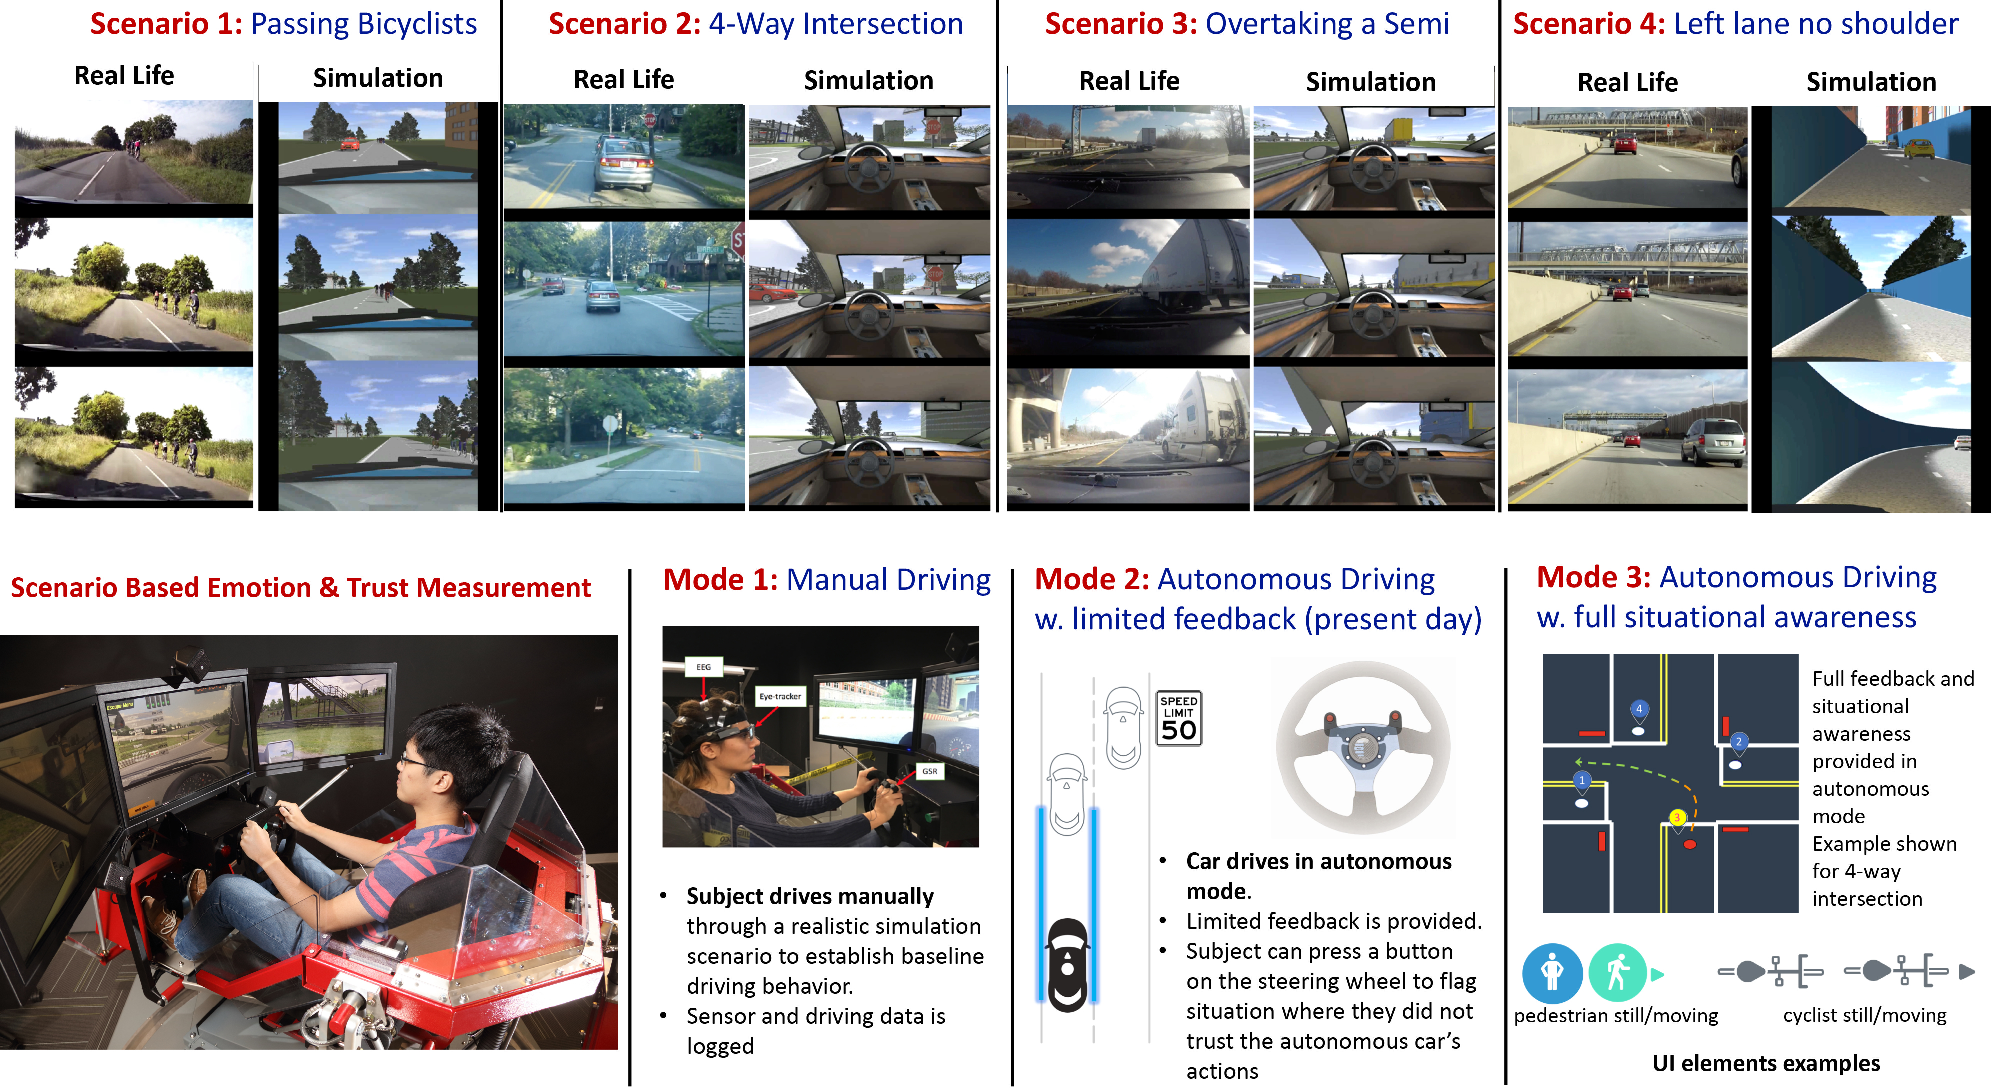
\includegraphics[width=0.7\columnwidth]{figures/scenarios.pdf}
    \caption{ We recreate real world traffic situations in simulation using PreScan. During experimentation, we invite human drivers to first manually drive through each scenario (mode 1), followed by an autonomous driving mode where limited feedback and car intentions are provided to the driver, and finally in mode 3, the users experience fully autonomous driving with full feedback and situational awareness provided. We then survey the participants about what feedback enables their trust, which UI elements do they prefer, which mode made them emotionally satisfied.  }
    \label{fig:scenario}
\end{figure}

Behind the wheels of a self-driving car, everyone becomes a backseat driver. For thrust 1 on monitoring driver behavior and emotions (Section~\ref{sec:behaviour}, we want to observe and record driver activity in a controlled environment. 
For thrust 3 on feedback design (Section~\ref{sec:feedback}), we want to measure how passengers react to varying degrees of feedback and explanations provided to them by the UI. 
We setup realistic traffic scenarios in our full scale driving simulator and run experiments to gather the data required to build models for human behavior, and test the effectiveness of different kinds of feedback. 
We have created four scenarios in our preliminary work – a four way stop sign, safely passing bicyclists, overtaking a large semi, driving close to a barrier in the absence of a shoulder.
\newline
\noindent[\textbf{Participants}]
We are proposing to conduct user studies and driving experiments for Thrusts 1, and 3.
The design of a subject study protocol is being undertaken at the time of writing this proposal. 
We are working with the Institutional Review Board for Social and Behavioral Sciences at the University of Virginia. 
The data management plan describes in detail how user data will be recorded, used, distributed, and maintained. 
A total of at least 100 participants from the University of Virginia will be recruited for participation in this study over 3 years. 
%We we take measures to ensure sufficient diversity within the participation pool. 
%Subjects will be awarded in exchange for participation in accordance with the University of Virginia’s Institutional Review Board practices, and we have requested a budget for the same.
\newline
\noindent[\textbf{Setup}]
Figure~\ref{fig:scenario} shows the full driving scale setup in Co-PI Feng's lab. 
The hardware platform is based on the Force Dynamics 401CR driving simulator - complete with pitch, roll, yaw, and heave, to simulate the experience of being in a vehicle. We expect to collect data about realistic human response during the driving. The driving simulation software is called PreScan, which is a software tool used by the industry for Advanced Driver Assistance Systems (ADAS) development. 
%PreScan supports virtual sensor technologies such as radar, laser, camera, ultrasonic, GPS and C2C/C2I communications. 
Sensors will be used for both high-level inference of human's intent and preferences and low-level monitoring of human behavioral, mental, and physiological states. These include EEG, EKG, EMG, cameras, eye tracking sensor, and cloud-based speech recognizers.
\newline
\noindent[\textbf{Design and procedure}]
As shown in Fig.~\ref{fig:scenario}, we have re-created 4 real world driving situations in Pre-Scan.
For each of these scenarios, we will conduct the following user experiment:
\begin{enumerate}[itemsep=0pt,parsep=0pt,topsep=4pt,leftmargin=0.4in]
    \item \textbf{Mode 1 - Manual driving}: In this mode, we ask the subject to manually drive through a given scenario. 
    %Each scenario's simulation is a few minutes. 
    As they drive through a scenario, we monitor the person's behavior and emotional cues as well as log their driving behavior to establish a baseline. 
    %This driving behavior ( steering, brake, acceleration) can be considered as their baseline profile. 
    %We also track their gaze, to asses what the driver is paying attention to as they drive. 
    As an example, we will ask the subject to drive through the four way stop sign scenario, where they have to self-asses their right of way as they approach a stop sign. We can then intentionally program one of the agents in the simulation to drive out of the order for the right of way and observe how the driver adapts. 
    \item \textbf{Mode 2 - Autonomous driving with limited feedback:} Next, we ask the same subject to sit back and relax, as the car drives by itself in autonomous mode. Everything in the scenario is identical to Mode 1, except that the driving is fully autonomous. We present the driver with a virtual dashboard which depicts what the car sees, very similar to the dashboards for semi-autonomous vehicles on the market today.  We monitor the drivers behavioral and emotional cues to interpret their trust in the system. We also give them the option to press a button on the steering wheel, every time they think the car did something that they did not anticipate, or if they mistrusted the car's autonomous driving actions. Flagging events in a scenario provides us with a basis for designing UI feedback later.
    %Continuing with our previous example, a visualization of the four way stop sigh is shown the viewer as feedback, but no indication is given as to if the autonomous car has figured out its right of way, or what is its intended trajectory.
    \item \textbf{Mode 3 - Autonomous driving with full feedback:} Finally, we have the autonomous car drive through the same scenario one more time, but this time we provide full situational awareness of the scene to the user along with cues about the car's intended actions. In the stop sign example, we project the car's understanding of its right of way, and how that dynamically updates as other vehicles drive through the intersection. We project the cars intended trajectory so the user know that the car will make a left turn and will yield to incoming traffic. For the parts of the simulation which were flagged by the user, we run the Deep Explanations engine to provide natural language explanations for the car's actions. 
\end{enumerate}
Following the experiment, we survey the subjects to understand and gather data on which explanations helped increase their trust, which UI elements worked, and to what extent.
Each participant will be given a questionnaire, adapted from~\cite{merritt2013trust}, to learn about their levels of trust in the autonomous car. 
%We will use scales which empirically define the feeling of trust in the autonomous system from~\cite{jian2000foundations} which has been used in many studies about trust~\cite{hoff2015trust}.
% \vspace{-5pt}
% \subsubsection{Expected results} 
%Upon the completion of data collection, it will be subjected to a factor analysis to reveal the underlying causes for trust and confusion.
% The goal of factor analysis is to condense a larger set of variables to a smaller set of factors, which account for a sizeable proportion of variability within the items. Thus, it is desirable to have a few factors that account for a large portion of the variance. 
% A one-way analysis of variance (ANOVA) will also be conducted to examine differences in trust amongst the different driving modes. 
% It is anticipated that there will be differences in trust depending on the subject's preferences, driving style, and the autonomous car's behavior. 
% More specifically, we anticipate that trust will attenuate with higher levels of feedback. We will create a library of UI elements, a library of simulation scenarios, with detailed statistics about which elements worked and what was the subject's assesment.
\newline
\noindent[\textbf{Expected Results}] The scenario based experimentation will enable creating a library of emotional profiles, and models of drivers; identify the mapping between the emotional states and the driving preferences, collect valuable data for training the Deep Explanations networks for natural language feedback; and by deploying the same subject in a real car and monitoring their preferences and driving behavior, we will also validate the realism of the simulation study. 
The simulation setup offers a distinct advantage, i.e. repeatability of the same scenario, however as explained in Thrust 1 (Section~\ref{sec:behaviour}) - to develop the proposed models for emotion and driving behavior, data from real deployment in subject-owned vehicles will be used . 


